% igs2ejournalguide.tex
% v4.00 3-sept-2015

\NeedsTeXFormat{LaTeX2e}

% check that the math fits the two-column format:
% \documentclass[twocolumn]{igs}

% but use this version when submitting your article:
  \documentclass[review,oneside]{igs}

% other options are available
%   authors printing on US letter size are advised 
%   to use the slightly shorter [letterpaper] option
% SINGLE COLUMN
%   \documentclass{igs}              
% SINGLE COLUMN, FEWER LINES/PAGE
%   \documentclass[letterpaper]{igs} 
% DOUBLE COLUMN, FEWER LINES/PAGE
%   \documentclass[twocolumn,letterpaper]{igs} 

  \usepackage{igsnatbib}

% check if we are compiling under latex or pdflatex
  \ifx\pdftexversion\undefined
    \usepackage[dvips]{graphicx}
  \else
    \usepackage[pdftex]{graphicx}
    \usepackage{epstopdf}
    \epstopdfsetup{suffix=}
  \fi

% the default is for unnumbered section heads
% if you really must have numbered sections, remove
% the % from the beginning of the following command
% and insert the level of sections you wish to be
% numbered (up to 4):

% \setcounter{secnumdepth}{2}

\begin{document}

\title[IGS \LaTeXe\ guide]{Journal of Glaciology 
  authors' guide to the IGS~\LaTeXe~class~file}

\author[Baxter and others]{Craig BAXTER,$^1$
  Rachel BROWN,$^2$\protect\thanks{Present address:
  Centre for Glaciology, Institute of Geography and
  Earth Sciences, University of Wales, Aberystwyth,
  UK.}\ \ Louise BUCKINGHAM,$^3$ 
  Magn\'us~M.~MAGN\'USSON$^1$}

\affiliation{%
$^1$International Glaciological Society, Scott
  Polar Research Institute, Cambridge, UK\\
$^2$Climate Change Institute, University of Maine,
  303 Bryand Global Sciences Center, Orono,
  ME, USA\\
$^3$Institute of Geological and Nuclear Sciences
  Ltd, Lower Hutt, New Zealand\\
  Correspondence: Craig Baxter 
  $<$craig@igsoc.org$>$}

\abstract{The design for the \emph{Journal of Glaciology} has been implemented as a \LaTeXe\ class file and is derived from article.cls. We recommend that authors use this guide as a template. Import your text to below the \texttt{\textbackslash maketitle} command and then cut-and-paste the title/author/affiliation/abstract details. While writing we suggest you use the two-column \texttt{[twocolumn]} option to check that mathematical equations fit the measure. Submitted papers must, however, be presented using the one-column \texttt{[review]} option. The \emph{Journal of Glaciology} is printed in Optima. However, submissions using Computer Modern are fine. If you have any problems using the class file, please email Craig Baxter at the above address, attaching your tex, log, cls, sty, bib, bbl, bst and any additional sty files you are using. The abstract should be less than 200 words and one paragraph long.}

\maketitle

\section{Using the IGS class file}
Please ensure you have downloaded the latest version from http:/$\!$/igsoc.org/production/. The IGS \LaTeXe\ journal guide has examples of most environments authors are likely to come across. The title page contains some new environments, e.g. affiliation and abstract. Papers should be divided into unnumbered sections with short section headings. SI units and internationally recognized systems of abbreviation should be used throughout. The \TeX\ file should be named to reflect your paper number, i.e. 15J299.tex. Please remove any extraneous text (e.g. text from previous drafts, notes and comments that will not form part of the final printed text of the paper).

\subsection{Additional packages supplied with igs.cls}
The distribution package contains the following files; the first 10 are IGS-specific, the other 10 are standard \LaTeX\ distribution files:\\[-0.5\baselineskip]
\begin{description}
\item [\texttt{igs2ejournalguide.tex}]\enskip   IGS \LaTeX\ guide
\item [\texttt{igs2ejournalguide.pdf}]\enskip   pdf file of this guide
\item [\texttt{igs2ejournalguide[twocolumn].pdf}]\enskip pdf file of this guide using the \verb"[twocolumn]" option
\item [\texttt{15J299Fig01.eps}]\enskip         Fig.~1 in this guide
\item [\texttt{15J299Fig02.eps}]\enskip         Fig.~2 in this guide
\item [\texttt{igs.cls}]\enskip                 IGS class file
\item [\texttt{igs.bst}]\enskip                 IGS bibliography style file
\item [\texttt{igsnatbib.sty}]\enskip           IGS style file for citations
\item [\texttt{igsupmath.sty}]\enskip           IGS style file for upright Greek characters
\item [\texttt{igsrefs.bib}]\enskip             sample \textsc{Bib}\TeX\ database
\item [\texttt{amsbsy.sty}]\enskip              style file called in by igsupmath.sty
\item [\texttt{amsfonts.sty}]\enskip            style file called in by amssymb.sty
\item [\texttt{amsgen.sty}]\enskip              style file called in by igsupmath.sty
\item [\texttt{amssymb.sty}]\enskip             accesses AMS fonts \verb"msam" and \verb"msbm"
\item [\texttt{ednmath0.sty}]\enskip            style file required for [review] option
\item [\texttt{edtable.sty}]\enskip             style file required for [review] option
\item [\texttt{graphicx.sty}]\enskip            graphics style file
\item [\texttt{lineno.sty}]\enskip              style file required for [review] option
\item [\texttt{ltabptch.sty}]\enskip            style file required for [review] option
\item [\texttt{vplref.sty}]\enskip              style file required for [review] option
\end{description}

\subsection{Typesetting the title page}

In the IGS design, shortened versions of the title and authors are used in the running head. The shortened version is specified in square braces immediately after the \verb"\title" and \verb"\author" commands (see below). The order in which the following elements appear may be crucial, i.e. \verb"\maketitle" must be the last command before your paper commences. 
The \emph{Journal of Glaciology} is printed on A4 paper which is slightly longer than US letter size. The default here is A4 paper but there is also a \verb"[letterpaper]" option. Be aware that using \verb"[letterpaper]" will fractionally lengthen your article. This guide was typeset using the following code:
\begin{verbatim}

% check that the math fits the two-column format:
% \documentclass[twocolumn]{igs}

% but use this version when submitting your article:
  \documentclass[review,oneside]{igs}

% other options are available
%   authors printing on US letter size are advised 
%   to use the slightly shorter [letterpaper] option
% SINGLE COLUMN
%   \documentclass{igs}              
% SINGLE COLUMN, FEWER LINES/PAGE
%   \documentclass[letterpaper]{igs} 
% DOUBLE COLUMN, FEWER LINES/PAGE
%   \documentclass[twocolumn,letterpaper]{igs} 
   
  \usepackage{igsnatbib}

% check if we are compiling under latex or pdflatex
  \ifx\pdftexversion\undefined
    \usepackage[dvips]{graphicx}
  \else
    \usepackage[pdftex]{graphicx}
    \usepackage{epstopdf}
    \epstopdfsetup{suffix=}
  \fi

% the default is for unnumbered section heads
% if you really must have numbered sections, remove
% the % from the beginning of the following command
% and insert the level of sections you wish to be
% numbered (up to 4):

% \setcounter{secnumdepth}{2}

\begin{document}

\title[IGS \LaTeXe\ guide]{Journal of Glaciology 
  authors' guide to the IGS~\LaTeXe~class~file}

\author[Baxter and others]{Craig BAXTER,$^1$
  Rachel BROWN,$^2$\protect\thanks{Present address:
  Centre for Glaciology, Institute of Geography and
  Earth Sciences, University of Wales, Aberystwyth,
  UK.}\ \ Louise BUCKINGHAM,$^3$ 
  Magn\'us~M.~MAGN\'USSON$^1$}

\affiliation{%
$^1$International Glaciological Society, Scott
  Polar Research Institute, Cambridge, UK\\
$^2$Climate Change Institute, University of Maine,
  303 Bryand Global Sciences Center, Orono,
  ME, USA\\
$^3$Institute of Geological and Nuclear Sciences
  Ltd, Lower Hutt, New Zealand\\
  Correspondence: Craig Baxter 
  $<$craig@igsoc.org$>$}

\abstract{The design for the \emph{Journal of... 
The abstract should be less than 200 words and 
one paragraph long.}

\maketitle

\section{Using the IGS class file}

\end{verbatim}

\subsection{Lists}
The IGS class file provides for numbered (\verb"enumerate") and unnumbered (\verb"itemize") lists. Nested lists are not encouraged. The default numbering system is 1., 2., 3., etc.; please do not change this unless there is a good reason. The IGS design removes bullet points from unnumbered lists.

\subsection{User-defined macros}
If possible, please do not define any new macros.

\begin{table}% table1, one column
\caption{One-column table captions will extend beyond
  the rules in two-column format. Do not try to adjust!
  Table captions do not have full points at the end}
\label{period}
\begin{minipage}{86mm}% you only need this line if you
  % have a table footnote
\begin{tabular}{@{}lcc}\hline
Period\footnote{Please do not use more than one `\&' 
  between columns, and note that if a table includes 
  table footnotes, it must be inside a \texttt{minipage} 
  environment.}%
  & Surface elevation change
  & Emergence velocity\\ \hline
1975--85   & $-0.50$ & 0.43\\
1986--2002 & $-1.03$ & 0.32\\
Difference & $-0.53$ & \llap{$-$}0.11
\end{tabular}
\end{minipage}% you only need this line if you have a
              % table footnote
\vspace\baselineskip\hrule % to separate verbatim from table
\vspace\baselineskip
\begin{verbatim}
\begin{table}% table1, one column
\caption{One-column table captions will extend beyond
  the rules in two-column format. Do not try to adjust!
  Table captions do not have full points at the end}
\label{period}
\begin{minipage}{86mm}% you only need this line if you
  % have a table footnote
\begin{tabular}{@{}lcc}\hline
Period\footnote{Please do not use more than one `\&' 
  between columns, and note that if a table includes 
  table footnotes, it must be inside a \texttt{minipage} 
  environment.}%
  & Surface elevation change
  & Emergence velocity\\ \hline
1975--85   & $-0.50$ & 0.43\\
1986--2002 & $-1.03$ & 0.32\\
Difference & $-0.53$ & \llap{$-$}0.11
\end{tabular}
\end{minipage}% you only need this line if you have a
              % table footnote
\end{table}
\end{verbatim}
\vspace\baselineskip\hrule % to separate verbatim from text
\end{table}

\subsection{Tables}

Tables may be typeset in either one- or two-column format. To typeset two-column format, add asterisks\\
(\verb"\begin{table*}...\end{table*}") as shown in Table~\ref{seasonal}. We may change the format in-house if necessary. Please avoid the use of colour or shading. Note that if you choose to refer to tables using labels, \verb"\caption" must precede \verb"\label", as in standard \LaTeX. Vertical rules are not house-style and will be removed. Note the use of the minipage environment in Table~\ref{period} which enables table footnotes to be output. If the table is two-column, use \texttt{\{178mm\}} instead of \texttt{\{86mm\}} on line~6. The source code for Tables~\ref{period} and~\ref{seasonal} is shown immediately below the tables.

\begin{table*}% table2, two column
\caption{Two-column table. Seasonal and annual SAT trends ($^\circ$C\,decade$^{-1}$) in the Arctic}
\label{seasonal}
% the following illustrates how to align columns on decimal points
% since all numbers are the same width in LaTeX, redefine a ? to take up the width of a number
% do not use if your table contains a genuine ?
\catcode`\?=\active \gdef?{\setbox0=\hbox{0}\hbox to\wd0{}}%
\setlength\tabcolsep{2.5pt}% column separation reduced from the default 6pt so the table fits the measure
\begin{tabular}{@{}l@{\hspace{20pt}}ccccc@{\hspace{20pt}}ccccc}\hline
Area                 & \multicolumn{5}{c}{1951--2005} & \multicolumn{5}{c}{1976--2005}\\[5pt]
                     & Dec--Feb       & Mar--May    & Jun--Aug  & Sep--Nov         & Annual
                     & Dec--Feb       & Mar--May    & Jun--Aug  & Sep--Nov         & Annual\\ \hline
Atlantic region      & 0.09           & 0.29 & 0.10 & 0.09 & 0.15 & 0.470 & ??0.60 & 0.45 & 0.53 & 0.59\\
Siberian region      & 0.12           & 0.29 & 0.04 & 0.17 & 0.16 & 0.08? & ??0.69 & 0.29 & 0.59 & 0.48\\
Pacific region       & 0.45           & 0.46 & 0.25 & 0.26 & 0.35 & 0.712 & ??1.08 & 0.27 & 0.66 & 0.52\\
Canadian region      & 0.16           & 0.12 & 0.14 & 0.30 & 0.18 & 0.20? & ??0.52 & 0.48 & 0.94 & 0.53\\
Baffin Bay region    & \llap{$-$}0.02 & 0.10 & 0.00 & 0.15 & 0.02 & 0.33? & ??0.62 & 0.51 & 0.80 & 0.57\\
Arctic 1             & 0.16           & 0.21 & 0.12 & 0.20 & 0.18 & 0.36? & 200.65 & 0.42 & 0.74 & 0.54\\
Arctic 2             & 0.22           & 0.29 & 0.14 & 0.14 & 0.19 & 0.38? & ??0.60 & 0.40 & 0.51 & 0.45\\
Arctic 3             & 0.28           & 0.31 & 0.14 & 0.13 & 0.21 & 0.42? & ?40.53 & 0.41 & 0.42 & 0.43\\
NH ($\mathrm{land}
  + \mathrm{ocean}$) & 0.13           & 0.13 & 0.10 & 0.10 & 0.12 & 0.27? & ??0.24 & 0.25 & 0.25 & 0.25\\
\hline
\end{tabular}
% turn off the category change, otherwise the ? won't appear in the verbatim environment below
\catcode`\?=11%
\vspace{0.25\baselineskip}
\begin{verbatim}
\begin{table*}% table2, two column
\caption{Two-column table. Seasonal and annual SAT trends ($^\circ$C\,decade$^{-1}$) in the Arctic}
\label{seasonal}
% the following illustrates how to align columns on decimal points
% since all numbers are the same width in LaTeX, redefine a ? to take up the width of a number
% do not use if your table contains a genuine ?
\catcode`\?=\active \gdef?{\setbox0=\hbox{0}\hbox to\wd0{}}%
\setlength\tabcolsep{2.5pt}% column separation reduced from the default 6pt so the table fits the measure
\begin{tabular}{@{}l@{\hspace{20pt}}ccccc@{\hspace{20pt}}ccccc}\hline
Area                 & \multicolumn{5}{c}{1951--2005} & \multicolumn{5}{c}{1976--2005}\\[5pt]
                     & Dec--Feb       & Mar--May    & Jun--Aug  & Sep--Nov         & Annual
                     & Dec--Feb       & Mar--May    & Jun--Aug  & Sep--Nov         & Annual\\ \hline
Atlantic region      & 0.09           & 0.29 & 0.10 & 0.09 & 0.15 & 0.470 & ??0.60 & 0.45 & 0.53 & 0.59\\
Siberian region      & 0.12           & 0.29 & 0.04 & 0.17 & 0.16 & 0.08? & ??0.69 & 0.29 & 0.59 & 0.48\\
Pacific region       & 0.45           & 0.46 & 0.25 & 0.26 & 0.35 & 0.712 & ??1.08 & 0.27 & 0.66 & 0.52\\
Canadian region      & 0.16           & 0.12 & 0.14 & 0.30 & 0.18 & 0.20? & ??0.52 & 0.48 & 0.94 & 0.53\\
Baffin Bay region    & \llap{$-$}0.02 & 0.10 & 0.00 & 0.15 & 0.02 & 0.33? & ??0.62 & 0.51 & 0.80 & 0.57\\
Arctic 1             & 0.16           & 0.21 & 0.12 & 0.20 & 0.18 & 0.36? & 200.65 & 0.42 & 0.74 & 0.54\\
Arctic 2             & 0.22           & 0.29 & 0.14 & 0.14 & 0.19 & 0.38? & ??0.60 & 0.40 & 0.51 & 0.45\\
Arctic 3             & 0.28           & 0.31 & 0.14 & 0.13 & 0.21 & 0.42? & ?40.53 & 0.41 & 0.42 & 0.43\\
NH ($\mathrm{land}
  + \mathrm{ocean}$) & 0.13           & 0.13 & 0.10 & 0.10 & 0.12 & 0.27? & ??0.24 & 0.25 & 0.25 & 0.25\\
\hline
\end{tabular}
\end{table*}
\end{verbatim}
\vspace\baselineskip\hrule % to separate verbatim from text
\end{table*}


\subsection{Figures}

Figures may be typeset in either one- or two-column format. One-column format allows up to 86$\,$mm (e.g. Fig.~\ref{tracks}); two-column format up to 178$\,$mm (e.g. Fig.~\ref{filters}). Please do not provide original graphics files in which the figure is a great deal larger or smaller than what you envisage will be the final printed size. To typeset two-column format, add asterisks (\verb"\begin{figure*}...\end{figure*}") as shown in Fig.~\ref{filters}. We may change the format in-house if necessary. Please note that if you choose to refer to figures using labels, \verb"\caption" must precede \verb"\label", as in standard \LaTeX. 

Please send one file for each figure (in other words do not use subfigures) and use a name that clearly identifies it (e.g. `15J299Fig03.eps').

In addition, figures should be eps, ai (illustrator), ps, tif, psd or pdf. Use strong black lines with a width of at least 0.75pt at final printed size (avoid tinting if possible) and SI units in labels. Lettering should ideally be Optima to match the final typeface; Arial or a similar sans serif font for a second choice. Aim to have the final-size lettering at 9pt, if possible. Figures should not be in boxes. The source code for Figs~\ref{tracks} and~\ref{filters} is shown immediately below the figures.


\subsection{Equations}

We are including some complex equations as examples. Equations should be checked for width using the \verb"[twocolumn]" option. Note the use of arrays in the following equation:
\begin{equation}
\label{arrayexample}
\alpha_{t_2}= \left\{%
  \begin{array}{ll}
    \alpha_{t_1} - a_1 [\ln (T+1)]
      \mathrm{e}^{(a_2\sqrt{n})}
      & \mbox{$n_\mathrm{d} > 0\enskip$ and
      $\enskip T > 0$}\\
    \alpha_{t_1} - a_3 \mathrm{e}^{(a_2\sqrt{n})}
      & \mbox{$n_\mathrm{d} > 0\enskip$ and
      $\enskip T < 0$}\\
    \alpha_{t_1} + a_4 P_\mathrm{s}
      & \mbox{$n_\mathrm{d} = 0$}
  \end{array}
\right.
\end{equation}
Equation~(\ref{arrayexample}) above used the following code:
\begin{verbatim}

\begin{equation}
\label{arrayexample}
\alpha_{t_2}= \left\{%
  \begin{array}{ll}
    \alpha_{t_1} - a_1 [\ln (T+1)]
      \mathrm{e}^{(a_2\sqrt{n})}
      & \mbox{$n_\mathrm{d} > 0\enskip$ and
      $\enskip T > 0$}\\
    \alpha_{t_1} - a_3 \mathrm{e}^{(a_2\sqrt{n})}
      & \mbox{$n_\mathrm{d} > 0\enskip$ and
      $\enskip T < 0$}\\
    \alpha_{t_1} + a_4 P_\mathrm{s}
      & \mbox{$n_\mathrm{d} = 0$}
  \end{array}
\right.
\end{equation}

\end{verbatim}
Equations should be aligned on the equals signs where possible. Equations that extend beyond the one-column measure should be turned over before an operator. Note the \verb"\skew4" command below which moves the bar over the $R$ to the right. The value generally varies between \verb"\skew1" and \verb"\skew5".
\begin{eqnarray}
\label{eqnarrayexample}
l_c &=& l_0 \left(\frac{\skew4\bar R_m}{R} \right)^2
  \psi^{\frac{P}{P_0\cos Z}}\nonumber\\
    &&  \mbox{}\times [\cos\beta\, \cos Z
    + \sin\beta\,\sin Z\,\cos(\psi_\mathrm{sun}
    - \psi_\mathrm{slope})]
\end{eqnarray}
Equation~(\ref{eqnarrayexample}) above used the following code:
\begin{verbatim}

\begin{eqnarray}
\label{eqnarrayexample}
l_c &=& l_0 \left(\frac{\skew4\bar R_m}{R} \right)^2
  \psi^{\frac{P}{P_0\cos Z}}\nonumber\\
    &&  \mbox{}\times [\cos\beta\, \cos Z
    + \sin\beta\,\sin Z\,\cos(\psi_\mathrm{sun}
    - \psi_\mathrm{slope})]
\end{eqnarray}

\end{verbatim}

\subsection{Typesetting upright Greek characters}

The \verb"igsupmath" package provides macros for upright lower-case Greek (\verb"\ualpha"--\verb"\uxi"), and for bold lower-case Greek (\verb"\ubalpha"--\verb"\ubxi"). The bold upright symbol \verb"\eta" has to be treated differently, in this case use \verb"\uboldeta".

To use the \verb"igsupmath" package, you need to have the AMS \verb"eurm/b" fonts installed.

The AMS packages are supplied from the AMS\,\LaTeX\ distribution. If you already have the AMS\,\LaTeX\ distribution installed, you can safely delete the \verb"ams*.sty" files (it is worth checking if the supplied files are newer). If you do not have them already, the latest AMS Fonts/AMS\,\LaTeX\ distributions can be found at http:/$\!$/ctan.org/.

For upright characters add a \verb"u", and for upright bold characters, \verb"ub", e.g.\\*[0.5\baselineskip]
\begin{tabular}{@{}ll@{\hspace{40pt}}ll}
$\ualpha$   & \verb"$\ualpha$"      &    $\ubalpha$ & \verb"$\ubalpha$"\\
$\ubeta$    & \verb"$\ubeta$"       &    $\ubbeta$ & \verb"$\ubbeta$"\\
$\ugamma$   & \verb"$\ugamma$"      &    $\ubgamma$ & \verb"$\ubgamma$"\\
$\udelta$   & \verb"$\udelta$"      &    $\ubdelta$ & \verb"$\ubdelta$"
\end{tabular}\\[0.5\baselineskip]
Authors who do not have this font are requested to key their articles using the commands above. The characters will be substituted automatically by the typesetter.

\subsection{Typesetting the partial symbol}

The \verb"igsupmath" package also provides \verb"\upartial" and \verb"\ubpartial".

Provided you have the AMS fonts, you can use the style file igsupmath.sty to typeset the partial symbol, e.g.\\*[0.5\baselineskip]
\begin{tabular}{@{}ll@{\hspace{40pt}}ll}
$\upartial$ & \verb"$\upartial$"    &    $\ubpartial$ & \verb"$\ubpartial$"\\
\end{tabular}


\subsection{Marginal notes}

The IGS class file\marginpar{Editor! Help!} redefines the \LaTeX\ command \verb"\marginpar". If you wish to add a marginal note such as the one alongside this text, you would key \verb"\marginpar{Editor! Help!}". Marginal notes will be removed before printing.

\subsection{References}

All citations in text should include the author name(s) and the year of publication (e.g. `Smith, 2014'; `Smith and Jones, 2014'; `Smith and others, 2015') and have an entry in the reference list. 

References should:
\begin{itemize}
\item be short;
\item be complete and accurate;
\item be arranged in alphabetical order by first author's surname;
\item include too much rather than too little information;
\item include doi numbers where available (note that older bib databases often included doi's in the page field -- in which case they may appear after a comma and without braces);
\item include works accepted but not published as `in press';
\item not include personal communications, unpublished data or manuscript in preparation or submitted for publication, data published on the web (these should be included in the text).
\end{itemize}

\begin{figure}%fig1, one column
\centering{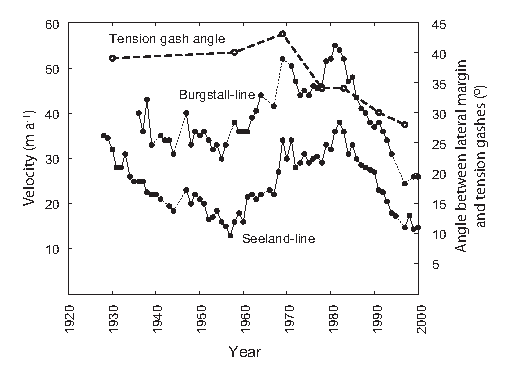
\includegraphics{15J299Fig01.eps}}
\caption{One-column figures should be $\leq$86$\,$mm.
Good artwork can make or break a paper. Capitalize
the first word of a label and use round not square 
brackets for units.}
\label{tracks}
\vspace\baselineskip\hrule % to separate figure from verbatim
\vspace\baselineskip
\begin{verbatim}
\begin{figure}%fig1, one column
\centering{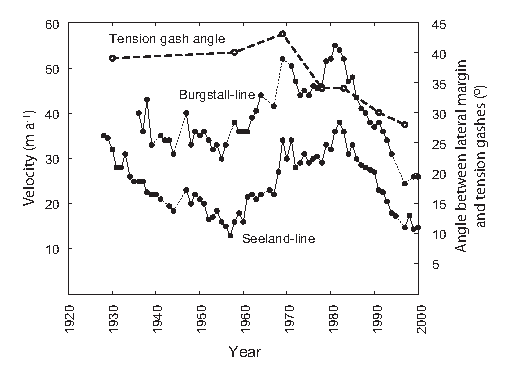
\includegraphics{15J299Fig01.eps}}
\caption{One-column figures should be $\leq$86$\,$mm.
Good artwork can make or break a paper. Capitalize
the first word of a label and use round not square 
brackets for units.}
\label{tracks}
\end{figure}
\end{verbatim}
\vspace\baselineskip\hrule % to separate verbatim from text
\end{figure}

\subsubsection{Automatic references using \textsc{Bib}\upshape{\TeX}}

To generate automatic references from a bib database, you must first specify the database (we are using \verb"igsrefs.bib") and then the IGS bibliography style by placing the following two commands where you would like the references to appear (normally at the end of your paper, before \verb"\end{document}"):
\begin{verbatim}

\bibliography{igsrefs}
\bibliographystyle{igs}

\end{verbatim}
%
Then run through the following steps:
\begin{enumerate}
\item Run your paper through \LaTeX.
\item Run \textsc{Bib}\TeX\ on your paper.
\item Open the newly-created bbl file containing the cited references and copy the entire contents to just below the \verb"bibliography"/\verb"bibliographystyle" commands.
\item Then comment them out:
\begin{verbatim}
%\bibliography{igsrefs}
%\bibliographystyle{igs}
\end{verbatim}
\item Run your paper through \LaTeX\ \textit{twice} more. 
\end{enumerate}
The IGS do not need your bib or bbl files. Note that \textsc{Bib}\TeX\ will lose the second initial in the entry `Box JE', for example, if it has been typed as `\{J.E.\} Box' in the bib file. This is because any text in an entry enclosed in \{\,\} will be treated as a single unit, and will not be further parsed. Prof. Box's name will typeset correctly if entered as `J. E. Box' in the bib file. 

If you have cited 16 references from the bib database, e.g. 
\citep{Rignot08},
\citep{Rignot08_2},
\citep{Motyka11},
\citep{Morlighem10},
\citep{Morlighem11},
\citep{Seroussi11},
\citep{Yan13},
\citep{Rogozhina12},
\citep{Hanna13},
\citep{Goelzer13},
\citep{Lucas12},
\citep{Edwards14},
\citep{gladstone_grl_10},
\citep{Morlighem13},
\citep{Goldberg11} and
\citep{paterson94}, the output will be just those 16 references and they will appear at the end of the article.

\paragraph{Citations using natbib commands}
Note that the standard natbib style file has been modified to fall into line with IGS style. The modified style file is called igsnatbib.sty (included in this distribution), and works exactly the same as natbib.sty. The default IGS house style is \citep{Yan13}. The following combinations are also available -- refer to the natbib documentation if you require any further explanation:\\*[0.5\baselineskip]
\begin{tabular}{@{}l@{\hskip -94pt}l}
\citep{Yan13}
    & \verb"\citep{Yan13}"\\
\citep[see][p.$\,$34]{Yan13}\\
    & \verb"\citep[see][p.$\,$34]{Yan13}"\\
\citep[e.g.][]{Yan13}
    & \verb"\citep[e.g.][]{Yan13}"\\
\citep[Section~2.3]{Yan13}\\
    & \verb"\citep[Section~2.3]{Yan13}"\\
\citep{Yan13, Edwards14}\\
    &  \verb"\citep{Yan13, Edwards14}"\\
\cite{Yan13, Edwards14}\\
    &  \verb"\cite{Yan13, Edwards14}"\\
\citealt{Yan13}
    & \verb"\citealt{Yan13}"\\
\cite{Yan13}
    & \verb"\cite{Yan13}"\\
\citealp{Yan13}
    & \verb"\citealp{Yan13}"\\
\citeauthor{Yan13}
    & \verb"\citeauthor{Yan13}"\\
\citeyearpar{Yan13}
    & \verb"\citeyearpar{Yan13}"\\
\citeyear{Yan13}
    & \verb"\citeyear{Yan13}"
\end{tabular}

\begin{figure*}%fig2, two column
\centering{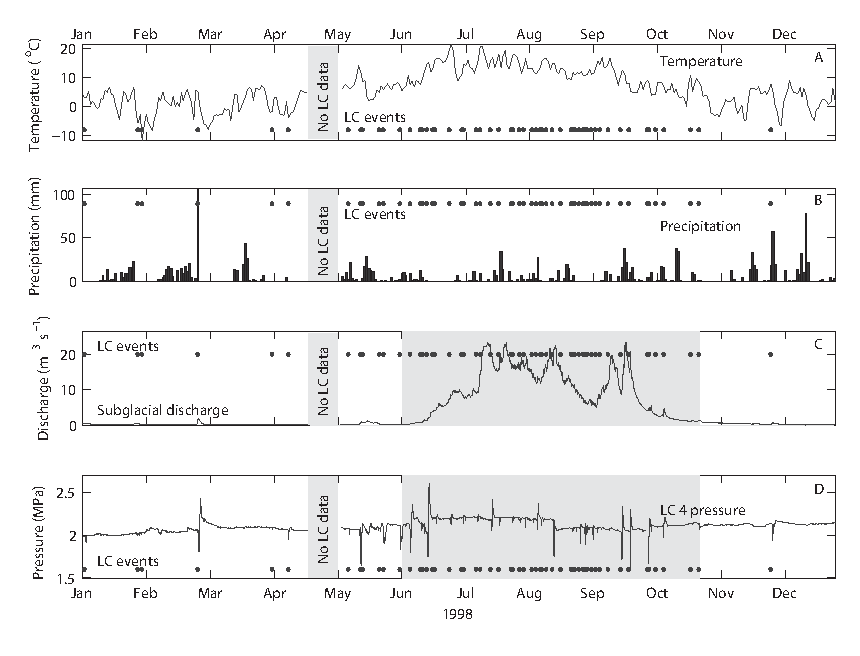
\includegraphics{15J299Fig02.eps}}
\caption{Two-column figures should be $\leq$178$\,$mm. SSA reconstructed components found by 
  projecting the SSA filters found using the whole 2000 traces in Fig.~4, on trace number 1, 
  ordered by magnitude of variance accounted for in the radar trace.}
\label{filters}
\vspace\baselineskip\hrule % to separate figure from verbatim
\vspace\baselineskip
\begin{verbatim}
\begin{figure*}%fig2, two column
\centering{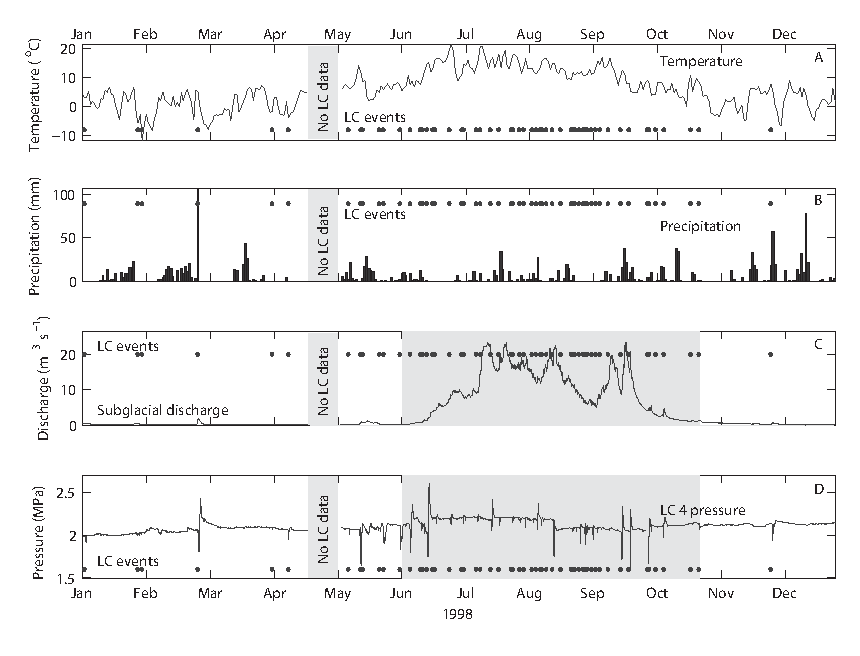
\includegraphics{15J299Fig02.eps}}
\caption{Two-column figures should be $\leq$178$\,$mm. SSA reconstructed components found by 
  projecting the SSA filters found using the whole 2000 traces in Fig.~4, on trace number 1, 
  ordered by magnitude of variance accounted for in the radar trace.}
\label{filters}
\end{figure*}
\end{verbatim}
\vspace\baselineskip\hrule % to separate verbatim from text
\end{figure*}

\subsubsection{Manual references}
References should be complete and conform to the IGS reference style. Particular points to note are that author names should be Surname followed by Initials, and that doi numbers, if available, must be included in parentheses at the end of the reference.
Authors not using the bibliography style file igs.bst can either produce a reference list in plain text or produce the same output at the end of the guide by typing the references along the following lines:

\begin{verbatim}

\begin{thebibliography}{16}
\providecommand{\natexlab}[1]{#1}
\expandafter\ifx\csname urlstyle\endcsname\relax
  \providecommand{\doi}[1]{doi: #1}\else
  \providecommand{\doi}{doi: \begingroup 
  \urlstyle{rm}\Url}\fi

\bibitem[\protect\citename{Edwards and others, }2014]
  {Edwards14}
  Edwards TL, Fettweis X, Gagliardini O, 
  Gillet-Chaulet F, Goelzer H, Gregory JM, Hoffman M, 
  Huybrechts P, Payne AJ, Perego M, Price S, 
  Quiquet A and Ritz C (2014) Effects of uncertainty 
  in surface mass balance-elevation feedback on 
  projections of the future sea level contribution 
  of the {G}reenland ice sheet. \emph{The Cryosphere}, 
  \textbf{8}, 195--208 (\doi {10.5194/tc-8-195-2014})

\bibitem[\protect\citename{Gladstone and others, }2010]
  {gladstone_grl_10}
  Gladstone RM, Lee V, Vieli A and Payne AJ (2010) 
  Grounding line migration in an adaptive mesh ice 
  sheet model. \emph{J. Geophys. Res.-Earth},
  \textbf{115}, F04014 (\doi {0.1029/2009JF001615})

\bibitem[\protect\citename{Goelzer and others, }2013]
  {Goelzer13}
  Goelzer H, Huybrechts P, F\"{u}rst JJ, Nick FM, 
  Andersen ML, Edwards TL, Fettweis X, Payne AJ and 
  Shannon S (2013) Sensitivity of {G}reenland ice
  sheet projections to model formulations. 
  \emph{J.~Glaciol.}, \textbf{59}(216), 733--749 
  (\doi {10.3189/2013JoG12J182})

\bibitem[\protect\citename{Goldberg and Sergienko, }2011]
  {Goldberg11}
  Goldberg DN and Sergienko OV (2011) Data assimilation 
  using a hybrid ice flow model. \emph{The Cryosphere}, 
  \textbf{5}, 315--327 (\doi {10.5194/tc-5-315-2011})

\bibitem[\protect\citename{Hanna and others, }2013]
  {Hanna13}
  Hanna E, Navarro FJ, Pattyn F, Domingues CM, 
  Fettweis X, Ivins ER, Nicholls RJ, Ritz C, Smith B, 
  Tulaczyk S, Whitehouse PL and Zwally HJ (2013) 
  Ice-sheet mass balance and climate change. \emph{Nature}, 
  \textbf{498}, 51--59 (\doi {10.1038/nature12238})

\bibitem[\protect\citename{Lucas-Picher and others, }2012]
  {Lucas12}
  Lucas-Picher P, Wulff-Nielsen M, Christensen JH, 
  Adalgeirsd\'ottir G, Mottram RH and Simonsen SB (2012) 
  Very high resolution regional climate model simulations 
  over Greenland: identifying added value. \emph{J.~Geophys.
  Res.}, \textbf{117}, D02108 (\doi {10.1029/2011JD016267})

\bibitem[\protect\citename{Morlighem and others, }2010]
  {Morlighem10}
  Morlighem M, Rignot E, Seroussi H, Larour E, Dhia HB 
  and Aubry D (2010) Spatial patterns of basal drag 
  inferred using control methods from a full-Stokes and 
  simpler models for Pine Island Glacier, West Antarctica.
  \emph{Geophys. Res. Lett.}, \textbf{37}, L14502 
  (\doi {10.1029/2010GL043853})

\bibitem[\protect\citename{Morlighem and others, }2011]
  {Morlighem11}
  Morlighem M, Rignot E, Seroussi H, Larour E, Dhia HB 
  and Aubry D (2011) A mass conservation approach for 
  mapping glacier ice thickness. \emph{Geophys. Res. Lett.}, 
  \textbf{38}, L19503 (\doi {10.1029/2011GL048659})

\bibitem[\protect\citename{Morlighem and others, }2013]
  {Morlighem13}
  Morlighem M, Seroussi H, Larour E and Rignot E (2013) 
  Inversion of basal friction in Antartica using exact 
  and incomplete adjoints of a higher-order model. 
  \emph{J.~Geophys. Res.}, \textbf{118}, 1746--1753 
  (\doi {10.1002/jgrf.20125})

\bibitem[\protect\citename{Motyka and others, }2011]
  {Motyka11}
  Motyka RJ, Truffer M, Fahnestock M, Mortensen J, 
  Rysgaard S and Howat I (2011) Submarine melting of 
  the 1985 Jakobshavn Isbrae floating tongue and the
  triggering of the current retreat. 
  \emph{J.~Geophys. Res.}, \textbf{116}, F01007 
  (\doi {10.1029/2009JF001632})

\bibitem[\protect\citename{Paterson, }1994]
  {paterson94}
  Paterson WSB (1994) \emph{The physics of 
  glaciers}. Butterworth-Heinemann, Oxford, 
  3rd edition

\bibitem[\protect\citename{Rignot and Steffen, }2008]
  {Rignot08}
  Rignot E and Steffen K (2008) Channelized bottom 
  melting and stability of floating ice shelves. 
  \emph{Geophys. Res. Lett.}, \textbf{35}, L02503 
  (\doi {10.1029/2007GL031765})

\bibitem[\protect\citename{Rignot and others, }2008]
  {Rignot08_2}
  Rignot E, Box JE, Burgess E and Hanna E (2008) 
  Mass balance of the Greenland ice sheet from 
  1958 to 2007. \emph{Geophys. Res. Lett.}, 
  \textbf{35}, L02502 (\doi {10.1029/2008GL035417})

\bibitem[\protect\citename{Rogozhina and others, }2012]
  {Rogozhina12}
  Rogozhina I, Hagedoorn JM, Martinec Z, Fleming K, 
  Soucek O, Greve R and Thomas M (2012) Effects of 
  uncertainties in the geothermal heat flux 
  distribution on the Greenland ice sheet: an 
  assessment of existing heat flow models.
  \emph{J.~Geophys. Res.}, \textbf{117}, F02025 
  (\doi {10.1029/2011JF002098})

\bibitem[\protect\citename{Seroussi and others, }2011]
  {Seroussi11}
  Seroussi H, Morlighem M, Rignot E, Larour E, 
  Aubry D, Dhia HB and Kristensen SS (2011) Ice flux 
  divergence anomalies on 79north glacier, Greenland.
  \emph{Geophys. Res. Lett.}, \textbf{38}, L09501 
  (\doi {10.1029/2011GL047338})

\bibitem[\protect\citename{Yan and others, }2013]
  {Yan13}
  Yan Q, Zhang Z, Gao Y, Wang H and Johannessan OM 
  (2013) Sensitivity of the modeled present-day 
  Greenland ice sheet to climatic forcing and 
  spin-up methods and its influence on future sea 
  level projections. \emph{J. Geophys. Res. Earth 
  Surf.}, \textbf{118}, 2174--2189 
  (\doi {10.1002/jgrf.20156})

\end{thebibliography}
\end{verbatim}

\section{Acknowledgements} 
We would like to thank Jason Amundson, Ed Bueler, Andrew Clifton, Gwenn~Flowers, Ralf Greve and Doug MacAyeal for their constructive reviews of the IGS class file and guide. Thanks are also due to Patrick Daly who once again helped to generate the latest version of igs.bst.

% authors generating their own bbl file would uncomment the following two lines, and comment out/delete the references below:

% \bibliography{igsrefs}   % reads igsrefs.bib
% \bibliographystyle{igs}  % imposes IGS bibliography style on output

% however, we are going to include igs2ejournalguide.bbl here:

\begin{thebibliography}{16}
\providecommand{\natexlab}[1]{#1}
\expandafter\ifx\csname urlstyle\endcsname\relax
  \providecommand{\doi}[1]{doi: #1}\else
  \providecommand{\doi}{doi: \begingroup 
  \urlstyle{rm}\Url}\fi

\bibitem[\protect\citename{Edwards and others, }2014]
  {Edwards14}
  Edwards TL, Fettweis X, Gagliardini O, 
  Gillet-Chaulet F, Goelzer H, Gregory JM, Hoffman M, 
  Huybrechts P, Payne AJ, Perego M, Price S, 
  Quiquet A and Ritz C (2014) Effects of uncertainty 
  in surface mass balance-elevation feedback on 
  projections of the future sea level contribution 
  of the {G}reenland ice sheet. \emph{The Cryosphere}, 
  \textbf{8}, 195--208 (\doi {10.5194/tc-8-195-2014})

\bibitem[\protect\citename{Gladstone and others, }2010]
  {gladstone_grl_10}
  Gladstone RM, Lee V, Vieli A and Payne AJ (2010) 
  Grounding line migration in an adaptive mesh ice 
  sheet model. \emph{J. Geophys. Res.-Earth},
  \textbf{115}, F04014 (\doi {0.1029/2009JF001615})

\bibitem[\protect\citename{Goelzer and others, }2013]
  {Goelzer13}
  Goelzer H, Huybrechts P, F\"{u}rst JJ, Nick FM, 
  Andersen ML, Edwards TL, Fettweis X, Payne AJ and 
  Shannon S (2013) Sensitivity of {G}reenland ice
  sheet projections to model formulations. 
  \emph{J.~Glaciol.}, \textbf{59}(216), 733--749 
  (\doi {10.3189/2013JoG12J182})

\bibitem[\protect\citename{Goldberg and Sergienko, }2011]
  {Goldberg11}
  Goldberg DN and Sergienko OV (2011) Data assimilation 
  using a hybrid ice flow model. \emph{The Cryosphere}, 
  \textbf{5}, 315--327 (\doi {10.5194/tc-5-315-2011})

\bibitem[\protect\citename{Hanna and others, }2013]
  {Hanna13}
  Hanna E, Navarro FJ, Pattyn F, Domingues CM, 
  Fettweis X, Ivins ER, Nicholls RJ, Ritz C, Smith B, 
  Tulaczyk S, Whitehouse PL and Zwally HJ (2013) 
  Ice-sheet mass balance and climate change. \emph{Nature}, 
  \textbf{498}, 51--59 (\doi {10.1038/nature12238})

\bibitem[\protect\citename{Lucas-Picher and others, }2012]
  {Lucas12}
  Lucas-Picher P, Wulff-Nielsen M, Christensen JH, 
  Adalgeirsd\'ottir G, Mottram RH and Simonsen SB (2012) 
  Very high resolution regional climate model simulations 
  over Greenland: identifying added value. \emph{J.~Geophys.
  Res.}, \textbf{117}, D02108 (\doi {10.1029/2011JD016267})

\bibitem[\protect\citename{Morlighem and others, }2010]
  {Morlighem10}
  Morlighem M, Rignot E, Seroussi H, Larour E, Dhia HB 
  and Aubry D (2010) Spatial patterns of basal drag 
  inferred using control methods from a full-Stokes and 
  simpler models for Pine Island Glacier, West Antarctica.
  \emph{Geophys. Res. Lett.}, \textbf{37}, L14502 
  (\doi {10.1029/2010GL043853})

\bibitem[\protect\citename{Morlighem and others, }2011]
  {Morlighem11}
  Morlighem M, Rignot E, Seroussi H, Larour E, Dhia HB 
  and Aubry D (2011) A mass conservation approach for 
  mapping glacier ice thickness. \emph{Geophys. Res. Lett.}, 
  \textbf{38}, L19503 (\doi {10.1029/2011GL048659})

\bibitem[\protect\citename{Morlighem and others, }2013]
  {Morlighem13}
  Morlighem M, Seroussi H, Larour E and Rignot E (2013) 
  Inversion of basal friction in Antartica using exact 
  and incomplete adjoints of a higher-order model. 
  \emph{J.~Geophys. Res.}, \textbf{118}, 1746--1753 
  (\doi {10.1002/jgrf.20125})

\bibitem[\protect\citename{Motyka and others, }2011]
  {Motyka11}
  Motyka RJ, Truffer M, Fahnestock M, Mortensen J, 
  Rysgaard S and Howat I (2011) Submarine melting of 
  the 1985 Jakobshavn Isbrae floating tongue and the
  triggering of the current retreat. 
  \emph{J.~Geophys. Res.}, \textbf{116}, F01007 
  (\doi {10.1029/2009JF001632})

\bibitem[\protect\citename{Paterson, }1994]
  {paterson94}
  Paterson WSB (1994) \emph{The physics of 
  glaciers}. Butterworth-Heinemann, Oxford, 
  3rd edition

\bibitem[\protect\citename{Rignot and Steffen, }2008]
  {Rignot08}
  Rignot E and Steffen K (2008) Channelized bottom 
  melting and stability of floating ice shelves. 
  \emph{Geophys. Res. Lett.}, \textbf{35}, L02503 
  (\doi {10.1029/2007GL031765})

\bibitem[\protect\citename{Rignot and others, }2008]
  {Rignot08_2}
  Rignot E, Box JE, Burgess E and Hanna E (2008) 
  Mass balance of the Greenland ice sheet from 
  1958 to 2007. \emph{Geophys. Res. Lett.}, 
  \textbf{35}, L02502 (\doi {10.1029/2008GL035417})

\bibitem[\protect\citename{Rogozhina and others, }2012]
  {Rogozhina12}
  Rogozhina I, Hagedoorn JM, Martinec Z, Fleming K, 
  Soucek O, Greve R and Thomas M (2012) Effects of 
  uncertainties in the geothermal heat flux 
  distribution on the Greenland ice sheet: an 
  assessment of existing heat flow models.
  \emph{J.~Geophys. Res.}, \textbf{117}, F02025 
  (\doi {10.1029/2011JF002098})

\bibitem[\protect\citename{Seroussi and others, }2011]
  {Seroussi11}
  Seroussi H, Morlighem M, Rignot E, Larour E, 
  Aubry D, Dhia HB and Kristensen SS (2011) Ice flux 
  divergence anomalies on 79north glacier, Greenland.
  \emph{Geophys. Res. Lett.}, \textbf{38}, L09501 
  (\doi {10.1029/2011GL047338})

\bibitem[\protect\citename{Yan and others, }2013]
  {Yan13}
  Yan Q, Zhang Z, Gao Y, Wang H and Johannessan OM 
  (2013) Sensitivity of the modeled present-day 
  Greenland ice sheet to climatic forcing and 
  spin-up methods and its influence on future sea 
  level projections. \emph{J. Geophys. Res. Earth 
  Surf.}, \textbf{118}, 2174--2189 
  (\doi {10.1002/jgrf.20156})

\end{thebibliography}

\appendix
\section{Appendix}

Start an appendix by \hbox{typing \verb"\appendix\section{Appendix}".} Appendices appear after the references. Equation numbers automatically start again with (\ref{appeqn}).
\begin{equation}
\label{appeqn}
 2\eta\kappa \frac{\partial \skew1\bar u}{\partial t} + \rho_{\mathrm r} g \skew1\bar u + D\kappa^4 \skew1\bar u = \skew3\bar\sigma_{zz}.
\end{equation}

\section{Handling more than one appendix}
Use the following code to achieve heading APPENDIX~A followed by APPENDIX~B and APPENDIX~C, with appropriate equation numbers:

\begin{verbatim}

\appendix
\section{Appendix A}

\setcounter{equation}{0}
\renewcommand\theequation{B\arabic{equation}}
\section{Appendix B}

\setcounter{equation}{0}
\renewcommand\theequation{C\arabic{equation}}
\section{Appendix C}
\end{verbatim}

\end{document}
